%!TEX program = pdflatex
\documentclass[conference,10pt,a4paper]{IEEEtran}

\usepackage{ifluatex}
\ifluatex
  \usepackage{fontspec}
  \usepackage{polyglossia} % babel replacement for use with fontspec
  \setdefaultlanguage[variant=american]{english}
  \selectlanguage[variant=american]{english}
\else
  \usepackage[utf8]{inputenc}
  \usepackage[T1]{fontenc}
  \usepackage[american]{babel}
\fi

\usepackage[acronym, nomain, nowarn]{glossaries}
\loadglsentries{acronyms}
\usepackage{csquotes}
\usepackage{booktabs}
\usepackage[hyphens]{url}
\usepackage[pdfhighlight=/O, hidelinks, unicode=true]{hyperref}
\usepackage{mathtools}
\usepackage{fixmath}
\usepackage{algorithm2e}
\usepackage{subcaption}
\usepackage[load-configurations={abbreviations,binary}, per-mode=symbol]{siunitx}
\sisetup{load-configurations = abbreviations,binary-units}
\usepackage{tabu}
\makeglossaries
\usepackage[url=false,doi=false,backend=biber,style=ieee,isbn=false,sorting=none,minnames=1,maxnames=6]{biblatex}
\addbibresource{literature.bib}
\usepackage[inline]{enumitem}

\usepackage[np]{numprint}

\npstyleenglish

\newcommand{\hoss}[1]{\textcolor{red}{TH: #1}}

\makeatletter
\newcommand{\removelatexerror}{\let\@latex@error\@gobble}
\makeatother

% masks an issue with polyglossia, not sure of side effects
\AtBeginDocument{\let\textlabel\label}

\begin{document}

\title{The Cost of Cloud Gaming: Do the Benefits Outweigh the Costs?}

\author{\IEEEauthorblockN{Florian Metzger}
\IEEEauthorblockA{
Chair of Modeling of Adaptive Systems\\
University of Duisburg-Essen\\
Essen, Germany\\
florian.metzger@uni-due.de}
\and
\IEEEauthorblockN{a b}
\IEEEauthorblockA{
a\\
b\\
a.b@univie.ac.at}
\and
\IEEEauthorblockN{a b}
\IEEEauthorblockA{
a\\
b\\
a@informatik.uni-wuerzburg.de}}


\newcommand{\myparagraph}[1]{\subsubsection{#1}}

\maketitle

%%!TEX root = paper.tex
%%%%%%%%%%%%%%%%%%%%%%%%%%%%%%%%%%%%%%%%%%%%%%%%%%%%%%%%%%%%%%%%%%%%%%%%%%%%%%%%
\begin{abstract}

%stagnate in terms of commercial success. 
In recent years, cloud gaming has become a popular research topic, and the list of its supposed benefits is long. However, cloud gaming platforms are still waiting for the commercial breakthrough. This might be caused by the pricing models and product offerings by existing ``à la carte'' platforms. This paper aims at investigating the costs and benefits of both platform types through a twofold approach. We first take on the perspective of the customers, and investigate several cloud gaming platforms and their pricing models in comparison to the costs of ``à la carte'' platforms. Then, we explore engagement metrics in order to assess the enjoyment of playing the offered games. Lastly, coming from the perspective of the service providers, we aim to give reasons for the problematic nature of operating a large-scale cloud gaming service while maintaining high \acrshort{QoE} values. Our analysis provides initial, yet still comprehensive reasons and models for the prospects of cloud gaming in a highly competitive market.

\end{abstract}

%%!TEX root = paper.tex
%%%%%%%%%%%%%%%%%%%%%%%%%%%%%%%%%%%%%%%%%%%%%%%%%%%%%%%%%%%%%%%%%%%%%%%%
%%%%%%%

\todo[inline,color=red!10]{Other title could be: The Prospects of Cloud 
Gaming: Do ... }

\section{Introduction}

Cloud gaming has become quite a popular research topic in recent years. 
Much of this research is aimed at comparing the experienced 
quality of cloud gaming to that of conventional gaming approaches, with 
the results
% Albert: even in terms of cost effectiveness, potential choice of 
% games, lower demands on required end user hardware
% (AKA the usual cloud gaming selling points)?
generally in favor of conventional gaming, but only by a 
tiny margin. Some publications even praise the method and attest high 
\gls{QoE} values.

So, if there are only negligible quality drawbacks --- according to the 
literature --- what about the commercial success of cloud gaming? In 
theory, there could be large economic benefits for users that should 
foster a quick adaptation of such services. 
However, quite a few commercial services have already come and gone, 
with a rather high rate of fluctuation. For example, one of the most 
prominent services in the past, \textsc{OnLive}, shut down and was forced to 
sell off its remaining assets.

All cloud gaming services, current as well 
as past, come with some subtle differences in their service, including 
the technical aspects, the selection of games, and the pricing 
model.
Yet, differentiation has not helped to generate much more public 
interest either. 
This might be attributed to a circumstance that is easily  
overlooked when evaluating cloud gaming services: the strong 
competition with other non-cloud gaming platforms, such as the 
individual console platforms or the large market for PC games --- with the 
Steam\footnote{\url{http://store.steampowered.com/}} platform as one of 
its strongest contenders. The move to digital distribution has made the 
PC platform quite popular, and PC games pricing has become 
much more dynamic and affordable in the process.

On the surface, current Cloud Gaming services attempt to a adopt a 
\textit{fixed fee subscription} model over the traditional 
\textit{à la carte} model. 
This move proved to be hugely successful for other types of media, be 
it for example \textsc{Netflix} for movies and shows or 
\textsc{Spotify} for music. However, these two types of services seem 
to offer much more content at a comparable or even lower price point 
than Cloud Gaming services do. Additionally, the technical requirements 
to maintain a quality level on par with that of locally run games are 
also rather demanding.

The two main questions that this work aims to tackle are thus: 
\textit{``Can Cloud Gaming be attractive for users in today's highly 
competitive market?''} and \textit{``Can you operate a Cloud Gaming 
service with acceptable margins while maintaining acceptable quality 
levels?''}. Both questions are strongly intertwined as in order to make 
such services attractive one would have to offer sufficient quality and 
quantity of games with a competitive pricing while not operating at a 
loss. In practice one could actually simplify both questions quite 
easily to one: \textit{``Can you compete with the PC gaming and Steam 
ecosystem (in terms of quality, prices, and variety)?''}

In order to answer these questions, this paper looks at the perspective 
of users and service provider in separate and provides arguments backed 
by data and simple models. To investigate the customer's perspective we 
employ user domain-specific user engagement metrics --- amongst others 
review scores as well as the length and playtimes of games --- to 
compare various services --- Cloud Gaming as well as conventional --- 
to each other. Additionally, using this data some simple budget models 
are set up to compare what (in terms of the number and quality of 
games) for a certain amount of money. We find that in the investigated 
cases the Cloud Gaming services' offer is very limited yet still 
charges relatively high prices, thus limiting the attractiveness for 
users in comparison to alternative services.

Due to the limited amount of freely available data on operating a Cloud 
Gaming service, the perspective of the Cloud Gaming operator is 
investigated by setting up efficiency models centered around the 
overbooking rate. These initial figures highlight the problematic 
nature of Cloud Gaming in terms of scaling and cost efficiency. When 
compared to other cloud services, that achieve high values of cost 
efficiency and capacity utilization, we believe that Cloud Gaming 
platforms will be much more peak-oriented and can thus achieve much 
lower values of server utilization. The end-to-end lag requirements of 
games demand a server placement in the vicinity of the user and thus 
eliminate most multiplexing gains that a centralized data center can 
garner over the course of a day. Additionally, games require dedicated 
hardware support, which is of no much use to most other cloud use 
cases, diminishing the potential of cross-service reuse.

These initial insights do not shed a good light on the commercial 
future of Cloud Gaming services in general. Apart from achieving major 
cost reductions, while maintaining or better even improving streaming 
quality, the future of Cloud Gaming might be bleak. But there still 
might be some niches to place a Cloud Gaming service where the 
competition is less strong. We plan to take a deeper look at all these 
aspects and provide more detailed models in the future.

~\\
This paper is structured as follows. Sec.~\ref{sec:relatedwork} 
provides a brief overview of the related work. Afterwards, 
Sec.~\ref{sec:background} explains all the necessary terms and 
technical details to understand the topic. The main part of this work 
encompass Sections \ref{sec:engagement} and 
\ref{sec:suppliermodelling}, which conduct the dual-perspective 
investigation of the Cloud Gaming providers' and their competitions' 
business models and engagement from the angle of the user and the 
platform operator respectively. The paper concludes in 
Sec.~\ref{sec:conclusion} with some remarks and an outlook.

%%%%%%%%%%%%
% \subsection{Fragestellungen}

% \begin{itemize}
% 	\item Kostenmodell für Cloud Gaming Provider?
% 	\item Attraktivität für “Core Gamer”?
% 	\item Wieviel ist eine NutzerIn bereit für einen Streaming 
Service mit einem bestimmten Spieleangebot und einer bestimmten 
Streaming- Qualität (Video-Qualität, Latenz, Grafikeinstellungen des 
Spiels) zu zahlen?
% 	\item Can they be competitive against other gaming platforms, 
both from provider as well as customer perspective
% 			Most challenging: can it beat the Steam price 
model and quality/number of games? (plus bundle providers and sales)
% \end{itemize}
% Netflix-Analogie? 
%\input{big-picture}
%%!TEX root = paper.tex
%%%%%%%%%%%%%%%%%%%%%%%%%%%%%%%%%%%%%%%%%%%%%%%%%%%%%%%%%%%%%%%%%%%%%%%%%%%%%%%
\section{Related Work}


%%%%%%%%%%%%%%%%%%%%%%%%%%%%%%%%%%%%%%%%%%%%%%%%%%%%%%%%%%%%%%%%%%%%%%%%%%%%%%%
\section{Cost of Cloud Gaming}

``Mobile Cloud Gaming: Issues and Challenges'' \cite{Soliman2013}
short overview of some possible issues

``Will Mobile Cloud Gaming Work? Findings on Latency, Energy, and Cost'' \cite{Lampe:2013:MCG:2514943.2515398}
client-side costs (monetary, energy, latency) of mobile devices; however underestimates energy costs in comparison to local gaming, display is the biggest factor, which is not factored in (this factor is also the same in local as well as cloud gaming); the monetary cost factor also underestimates the contractual situation in countries like Germany
And despite all this, it still finds mobile cloud gaming rather unfeasible (except in WiFi)

``Where Did My Battery Go? Quantifying the Energy Consumption of Cloud Gaming'' \cite{6924295}
Similar notion as previous paper, more in-depth, focus only on energy costs
test impl of local running game artificially increases cpu/gpu load
especially for low load games only marginal energy savings for cloud approach (~12\%)
even best case (and unrealistically high load) only 38\% energy savings
considering all the other drawbacks that cloud streaming incurs, this might not be enough

``Measuring the Client Performance and Energy Consumption in Mobile Cloud Gaming'' \cite{Huang:2014:MCP:2755535.2755542}
Similar findings, only 30\% energy savings


``Cloud gaming: a green solution to massive multiplayer online games'' \cite{6882299}
(TODO: need to read the full text yet)
Argues that removing computation intense tasks from (mobile) user devices leads to overall energy savings


Also approaches that select (and cost-optimize the selection of) data-centers might not be applicable due to the stringent latency and BW requirements and the need for dedicated hardware (GPUs) and the statefulness of gaming, e.g.
``QoS-Aware, Cost-Efficient Selection of Cloud Data Centers'' \cite{6740249}
``Cost-efficient Capacitation of Cloud Data Centers for QoS-aware Multimedia Service Provision.'' \cite{hans2014cost} optimization to geographically clustered users
``Placing Virtual Machines to Optimize Cloud Gaming Experience'' \cite{6853364}
latter paper includes many server cost optimization parameters, that might be worth looking at

Another optimization TODO: read fulltext
``QoS-Aware Revenue-Cost Optimization for Latency-Sensitive Services in IaaS Clouds'' \cite{6365107}

%%%%%%%%%%%%%%%%%%%%%%%%%%%%%%%%%%%%%%%%%%%%%%%%%%%%%%%%%%%%%%%%%%%%%%%%%%%%%%%
\section{Cloud Gaming in General}


%%%%%%%%%%%%%%%%%%%%%%%%%%%%%%%%%%%%%%%%%%%%%%%%%%%%%%%%%%%%%%%%%%%%%%%%%%%%%%%
\section{QoS/QoE of Gaming in General}

``On the Impact of Delay on Real-time Multiplayer Games'' \cite{Pantel:2002:IDR:507670.507674}

``The Effects of Loss and Latency on User Performance in Unreal Tournament 2003'' \cite{Beigbeder:2004:ELL:1016540.1016556}

``An experimental estimation of latency sensitivity in multiplayer Quake 3'' \cite{1266180}

``QoE Assessment of Interactivity and Fairness in First Person Shooting with Group Synchronization Control'' \cite{Ida:2010:QAI:1944796.1944806}

``Assessing the Impact of Game Type, Display Size and Network Delay on Mobile Gaming QoE'' \cite{beyer2014typedisplaydelayimpact}

``Latency and Player Actions in Online Games'' \cite{Claypool:2006:LPA:1167838.1167860}

%%%%%%%%%%%%
\subsection{Models}
``A Comprehensive End-to-End Lag Model for Online and Cloud Video Gaming'' \cite{metzger16lagmodel}


%%%%%%%%%%%%
\subsection{Measurements and Methods}

``A Method For Feedback Delay Measurement Using a Low-cost Arduino Microcontroller'' \cite{beyermethod}

``Towards a New {ITU-T} Recommendation for Subjective Methods Evaluating Gaming {QoE}'' \cite{mollertowards}

``Effect of Network Quality on Player Departure Behavior in Online Games'' \cite{4591393}

``An Empirical Study of Cloud Gaming'' \cite{Manzano:2012:ESC:2501560.2501582}

%%%%%%%%%%%%
\subsection{Studies}

``How Sensitive Are Online Gamers to Network Quality?'' \cite{Chen:2006:SOG:1167838.1167859}

``A Measurement Study Regarding Quality of Service and Its Impact on Multiplayer Online Games'' \cite{Bredel:2010:MSR:1944796.1944797}

``Empirical study of subjective quality for Massive Multiplayer Games'' \cite{4604397}



%%%%%%%%%%%%%%%%%%%%%%%%%%%%%%%%%%%%%%%%%%%%%%%%%%%%%%%%%%%%%%%%%%%%%%%%%%%%%%%
\section{QoS/QoE of Cloud Gaming}



``Modeling and Characterizing User Experience in a Cloud Server Based Mobile Gaming Approach'' (Shaoxuan Wang, Sujit Dey): http://esdat.ucsd.edu/projects/gaming/papers/globecom09.pdf

``The Impact of Video Encoding Parameters and Game Type on QoE for Cloud Gaming: a Case Study using the Steam Platform'' \cite{slivarimpact}

``On frame rate and player performance in first person shooter games'' \cite{claypool2007}


%%%%%%%%%%%%
\subsection{Measurements and Methods}
``Using Electroencephalography and Subjective Self-Assessment to Measure the Influence of Quality Variations in Cloud Gaming'' \cite{beyerusing}

``Cloud gaming: architecture and performance'' \cite{6574660}

``Measuring the Latency of Cloud Gaming Systems'' \cite{Chen:2011:MLC:2072298.2071991}

``On the Quality of Service of Cloud Gaming Systems'' \cite{6670099}

``The Brewing Storm in Cloud Gaming: A Measurement Study on Cloud to End-user Latency'' \cite{Choy:2012:BSC:2501560.2501563}

%%%%%%%%%%%%
\subsection{Subjective Studies}

``Gaming in the clouds: QoE and the users’ perspective'' \cite{Jarschel20132883}

``Are all games equally cloud-gaming-friendly? An electromyographic approach'' \cite{6404025}

``Subjective Evaluation of Latency and Packet Loss in a Cloud-Based Game'' \cite{6614351}

``An Evaluation of {QoE} in Cloud Gaming Based on Subjective Tests'' \cite{5976180}

%%%%%%%%%%%%
\subsection{QoE Adaptations}

video rate adaptations
``Addressing Response Time and Video Quality in Remote Server Based Internet Mobile Gaming'' \cite{5506572}

``Adaptive Mobile Cloud Computing to Enable Rich Mobile Multimedia Applications'' \cite{6413270}




%%%%%%%%%%%%%%%%%%%%%%%%%%%%%%%%%%%%%%%%%%%%%%%%%%%%%%%%%%%%%%%%%%%%%%%%%%%%%%%
\section{Other}


High frame rates:
``The Application of Sampling Theory to Television Frame Rate Requirements''
\url{http://www.bbc.co.uk/rd/publications/whitepaper282}
``High Frame-Rate Television''
\url{http://www.bbc.co.uk/rd/publications/whitepaper169}
``Higher Frame rates for more Immersive Video and Television''
\url{http://www.bbc.co.uk/rd/publications/whitepaper209}


Fundamental findings on framerates
``Experimentelle Studien über das Sehen von Bewegung'' \cite{wertheimer1912experimentelle}

VR:
``How Do New Visual Immersive Systems Influence Gaming QoE?'' \cite{7148110}


Hybrid Cloud/Local
``Kahawai: High-Quality Mobile Gaming Using GPU Offload'' \cite{Cuervo:2015:KHM:2742647.2742657}


Speculative Rendering of Future Frames
``Outatime: Using Speculation to Enable Low-Latency Continuous Interaction for Mobile Cloud Gaming'' \cite{Lee:2015:OUS:2742647.2742656}

``Security issues in online games'' \cite{doi:10.1108/02640470210424455}




%%!TEX root = paper.tex
%%%%%%%%%%%%%%%%%%%%%%%%%%%%%%%%%%%%%%%%%%%%%%%%%%%%%%%%%%%%%%%%%%%%%%%%%%%%%%%
%\section{Cloud Gaming Provider Models}

\section{Supply-Side Efficiency Modelling} % OR ONLY: THE SUPPLIER'S PROBLEM

%%%%%%%%%%%%%%%%%%%%%%%%%%%%%%%%%%%%%%%%%%%%%%%%%%%%%%%%%%%%%%%%%%%%%%%%%%%%%%%

%\subsection{Computational Efficiency}

Based on the collected consumer price figures of Section XXX, this section will elaborate on the required computational efficiency, i.e., cost per hosted subscriber, in order to successfully establish cloud gaming approaches on the market. Due to the limited available data, this investigation will follow a one data center assumption. Due to the demands of cloud gaming to serve both high performance and low latency, regional data centers will play a dominant role in the provider side cost modelling. Following this assumption, hereinafter a specific model is created that characterises at which cost efficiency levels the cloud gaming business can be operated successfully.

\begin{figure}[!t]
	\centering
	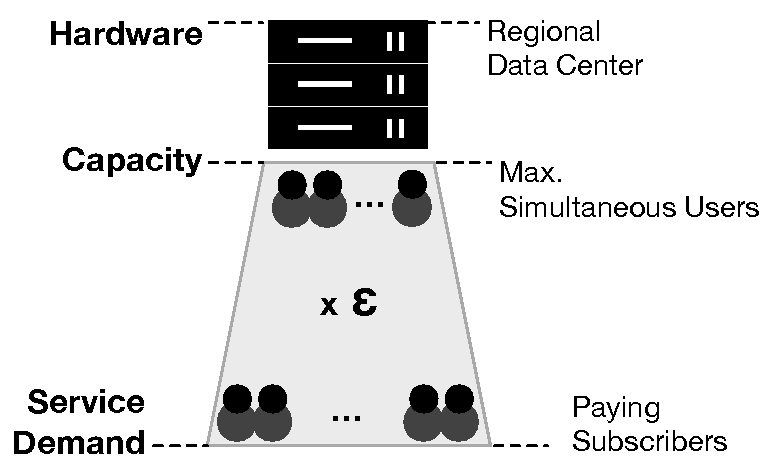
\includegraphics[width=0.65\columnwidth]{images/overbooking_datacenter.pdf}
	\caption{Overbooking of available computational capacity.}
\label{fig:overbooking_datacenter}
\end{figure}

The computational efficiency considers the maximum overbooking rate $\epsilon \geq 1$, where $\epsilon = 1$ refers to no overbooking. $\epsilon$ is calculated as ratio of the peak utilization $d_{peak}$ (number of peak time users) from the overall capacity $Cap$, 

\begin{equation}
	\epsilon = \frac{Cap}{d_{peak}} \quad ,
\end{equation}

where $Cap$ refers to the number of subscribed users that can be handled simultaneously by this data center. The maximum number of subscribers $d$ (maximum service demand) is, thus, given by

\begin{equation}
	 d = Cap \cdot \epsilon \quad .
\end{equation}

The average monthly customer price $\bar{p}$ aggregates the monthly subscription fee and the customer's depreciation costs for the hardware investments on a four years investment duration. We further consider a minimum profit margin $m$ of $3 \%$, which is in line with the average figure for the global game industry\footnote{\url{http://www.polygon.com/2012/10/1/3439738/the-state-of-games-state-of-aaa}} and substantially below the cloud computing figures that can range up to $16.9\%$\footnote{\url{http://www.forbes.com/sites/georgeanders/2015/04/23/amazons-web-services-delight-16-9-margins-more-joy-ahead/\#73324aa64b4e}} and potentially even higher\footnote{\url{http://www.bloomberg.com/news/articles/2015-12-02/microsoft-should-disclose-cloud-revenue-margins-ballmer-says}}.

%Global Games statistics / billion revenues 2012-2016: http://newzoo.com/infographics/global-games-market-report-infographics-2013/
% Game industry = 3%: http://www.polygon.com/2012/10/1/3439738/the-state-of-games-state-of-aaa
% Game industry in the past (2009 – average console game with margin of 40%): http://www.businessinsider.com/casual-gaming-profit-margins-near-90-2009-10?IR=T
% Profit margins in cloud computing:
%	Amazon 16.9% (2015): http://www.forbes.com/sites/georgeanders/2015/04/23/amazons-web-services-delight-16-9-margins-more-joy-ahead/#73324aa64b4e
% 	Microsoft 44% (2015) -- questionable: http://www.bloomberg.com/news/articles/2015-12-02/microsoft-should-disclose-cloud-revenue-margins-ballmer-says

\begin{align} \label{eq:computational_efficiency}
	\frac{\epsilon \cdot Cap \cdot \bar{p}}{Cap} :=& \underbrace{\frac{C_{cap}}{Cap}}_{C_{u}} \cdot m =\\
	= C_{u} = \frac{C_{cap}}{Cap} :=& \epsilon \cdot \bar{p}
\end{align}

When treating the costs of the regional data center as blackbox (operational and capital costs for the data center, and required game licensing fees), the analysis can concentrate on the required capacity and licensing cost $C_{u}$ per connected user $u$.

%\begin{equation}
%	ce = \frac{C_{cap}}{Cap} \quad .
%\end{equation}

%%%%%%%%%%%%%%%%%%%%%%%%%%%%%%%%%%%%%%%%%%%%%%%%%%%%%%%%%%%%
%SOME DATA CONSIDERATIONS:
%According to http://venturebeat.com/2014/01/15/steam-has-75-million-registered-users-third-party-steam-controllers-and-other-tidbits-from-valves-dev-days/
% Customer base of Steam was 75 Million active users in 2014. 
% %Vermutlich Nutzerzahl mittlerweile hoeher. Schaetzungen waeren also konservativ ausgerichtet.
%According to http://store.steampowered.com/stats/?l=german
% Höchststand (simultaneous): 12 406 722 Nutzer maximal, Feb 13 - Feb 15
% Peak immer abends. Niedrigster Wert bei <7.5 Mio Nutzern
% => \epsilon von 75/12,406722 = 6,0451100621
% Eigentlich, da steam wächst, > 6 eine gute Annahme. Wir könnten versuchen Schranken zu definieren.
% Wenn wir annehmen, dass Skalierung gut funktioniert, benoetigen wir keinen Buffer. Sollen wir Buffer verwenden?
%%%%%%%%%%%%%%%%%%%%%%%%%%%%%%%%%%%%%%%%%%%%%%%%%%%%%%%%%%%%

\todo[inline]{NOW LET'S ADD THE DATA. Check the 12.4 Mio. E.g. user older data. Introduce customer base data and reasoning above. Illustrate that epsilon will be around 6.}

For obtaining the required minimum margin $m$, the capacity and licensing cost per user $ce$ needs to be below XXXXXXXX Euro. Considering a capacity $Cap$ for 12.4 Mio active users, this refers to a total capacity cost $C_{Cap}$ of XXXXX Euro.

The overbooking ratio $\epsilon$ could also be increased by models fostering the off-peak usage, e.g., off-peak subscriptions that only allow access to the platform outside peak hours. When considering a substantial increase of the $\epsilon$ to $1.5$---the realistic maximum when considering the high peak time centricity of the gaming use case---, we obtain a substantially lowered $C_{u}$ requirement of 

\todo[inline]{ADD DATA}

Due to the requirement of using special hardware that is focused on the gaming use case, hardware sharing with other cloud applications seems unrealistic. Thus, we can characterise that the successful will have a maximum $C_{u}$ in the following bounds:

\todo[inline]{XXX}

This maximum does not consider that the operator may not be able to fully utilize the available capacity or may not hold the optimal game licenses at all times. Thus, in practice, the required hardware costs per subscriber have to be lower than $C_{u}$ .

\todo[inline]{NOW LET'S INTERPRET IF THAT SOUNDS LIKE A HARD THING TO DO OR NOT. AND THERE WE GO.}




%\input{simulation}
%\input{game-classification}
%%!TEX root = paper.tex
%%%%%%%%%%%%%%%%%%%%%%%%%%%%%%%%%%%%%%%%%%%%%%%%%%%%%%%%%%%%%%%%%%%%%%%%%%%%%%%%
\section{Conclusion}
\label{sec:conclusion}

While cloud gaming is a topic of strong interest, it comes with a series of problems and limitations, both technical as well as economic in nature. With the conducted user-side analysis it is easy to see the different, curated nature of current cloud gaming services, with their narrow offer of hand-selected games, in the case of \psnow even catered to a specific audience. This limits the attractiveness of any such service, even without looking at more intricate engagement metrics which would require more data than what was available.

But also the operator-side reveals major problems due to the need for highly regional data-centers and special hardware. This eliminates any chance for the efficiency gains that general cloud services are intended for.

However, there might be some niches for specific games or audiences that could be sustained at reduced operational efforts. This might be an angle worth of investigation in the future, especially with better engagement metrics and more detailed models of gaming data center operations.

However, there might also be a simpler and economically more feasible alternative to cloud gaming: game streaming in the local network, which would combine the open market structures of conventional gaming platforms with the ease of use of having a small box in the living that one just can play games on without much thought to the underlying hardware.

\printbibliography 

\end{document}
